\section{Реализция отказоустойчивого хранилища}

Для реализации понадобилось написать хранилище, которое работает по двум протоколам одновременно: HTTP, RPC.
Как было сказано выше, первый нужен для взаимодействия с пользователем, второй для взаимодействия внутри кластера
между всеми его узлами.

Также была реализована консольная утилита для удобства в старте всех узлов кластера, просмотра статусов каждого узла и
остановка всех узлов с помощью написанного файла конфигурации.

\subsection{Демонстрация возможностей хранилища}

Исполняемый файл представляет программу, написанную на языке программирования Го, реализующая следующий функционал:

\begin{enumerate}
  \item Хранение данных в формате ключ-значение.
  \item Отказоустойчивость -- репликация репликационного лога на все узлы типа Follower.
  \item Персистентность -- сброс данных, накопившихся в оперативной памяти на диск, что дает возможность восстанавливать
        состояние узла.
  \item Снапшотинг -- приложение создает полную копию данных.
\end{enumerate}

Для того, чтобы скомпилировать программу, нужно воспользоваться утилитой Go и исполнить следующую команду из-под корня проекта:

\begin{lstlisting}[frame=rlbt,language=Bash,caption={Сборка проекта хранилища}]
go build -o ./bin/node ./cmd/storage/main.go
\end{lstlisting}

На рисунке~\ref{fig:fig2} представлен вывод команды help для исполняемого файла хранилища.

\begin{figure}
  \centering
  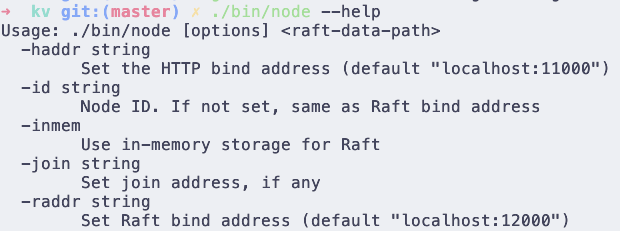
\includegraphics[scale=0.6]{assets/node.png}
  \caption{API для работы с бинарным файлом key-value хранилища}
  \label{fig:fig2}
\end{figure}

Программа предоставляет набор командных опций, которые используются для настройки и запуска узла в распределённом хранилище.
Ниже приведено описание доступных параметров командной строки:

\begin{itemize}
    \item \texttt{haddr string} \\
    Устанавливает HTTP-адрес, на котором будет доступен узел. По умолчанию значение — \texttt{localhost:11000}.
    
    \item \texttt{id string} \\
    Устанавливает идентификатор узла. Если не указан, используется значение, равное адресу привязки Raft.
    
    \item \texttt{inmem} \\
    Включает использование памяти для хранения данных Raft, вместо использования дискового хранилища.
    
    \item \texttt{join string} \\
    Устанавливает адрес узла (как правило он является лидером), к которому новый узел должен подключиться для вступления
    в кластер.
    
    \item \texttt{raddr string} \\
    Устанавливает адрес привязки для Raft. По умолчанию — \texttt{localhost:12000}.
\end{itemize}

Каждый из этих параметров настраивает различные аспекты поведения узла в кластерной системе, включая его сетевую доступность,
идентификацию в кластере и метод хранения данных.

Логи каждого узла хранятся по пути \texttt{{bin\_path}/{alias}/node.log}, где \texttt{bin\_path} и \texttt{alias} берyтся из конфига.
Наглядная демонстрация логирования приложения будет представлена в одном из следующих пунктов.

\subsection{Демонстрация возможностей кластерного менеджера}

Для того, чтобы не задумываться о каждом узле по отдельности, в частности, как запускать, следить за ним, было принято решение
реализовать консольную утилиту, которая по выданному конфигу, формат которого представлен в листинге~\ref{config} сможет стартовать
кластер одной командой, отслеживать статус всех инстансов хранилищ, а также останавливать кластер.

Утилита была написана с помощью фреймворка cobra, которая выделяется объемным функционалом, мощным инструментарием и легким
использованием.

Для того, чтобы скомпилировать программу, нужно воспользоваться утилитой Go и исполнить следующую команду из-под корня проекта:

\begin{lstlisting}[frame=rlbt,language=Bash,caption={Сборка консольной утилиты clusterctl}]
go build -o ./bin/clusterctl ./cmd/clusterctl/main.go
\end{lstlisting}

На рисунке~\ref{fig:fig2} представлен вывод команды help для исполняемого файла менеджера кластера.

\begin{figure}
  \centering
  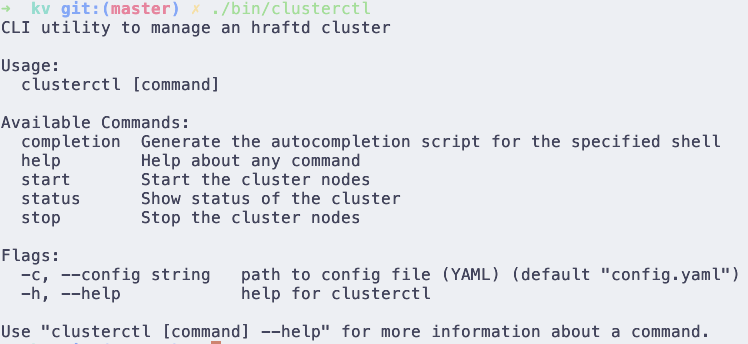
\includegraphics[scale=0.6]{assets/clusterctl.png}
  \caption{API для работы с бинарным файлом менеджера кластера}
  \label{fig:fig3}
\end{figure}

Программа предоставляет набор командных опций для управления кластером. Ниже приведены доступные команды и флаги:

\begin{itemize}
    \item \texttt{completion} -- генерирует скрипт автодополнения для указанной оболочки.
    
    \item \texttt{help} -- показывает справку по любой команде.
    
    \item \texttt{start} -- запускает узлы кластера согласно его конфигурации.
    
    \item \texttt{status} -- показывает статус активных узлов кластера и их роль (лидер или ведомый).
    
    \item \texttt{stop} -- останавливает узлы кластера.
\end{itemize}

Также доступны следующие флаги:
\begin{itemize}
    \item \texttt{-c, --config string} -- путь к файлу конфигурации в формате YAML (по умолчанию берется \texttt{config.yaml}
      в текущей директории).
    
    \item \texttt{-h, --help} -- показывает справку по программе.
\end{itemize}

\subsection{Дальнейшие шаги развития приложения}

Данная работа является наглядным примером работы алгоритма Raft и обладает минимально допустимым функционалом для хорошей демонстрации,
однако многих вещей не достает, что можно попытаться исправить в будущем.
Для дальнейшего развития программы можно выделить следующие направления:

\begin{itemize}
    \item Добавление команд в утилиту для управление кластером clusterctl. Например, реализация всех запросов (добавление, удаление, чтение) с
      данными на кластер, чтобы дополнительно не искать rw-инстанс (лидера).
    \item Улучшение логирования, использование более эффективных форматов хранения данных, таких как Protocol Buffers.
    \item Реализация автоматического восстановления узлов, поддержка мульти-кластерных развертываний для улучшения отказоустойчивости.
    \item Расширение API для более детализированного мониторинга и управления, интеграция с внешними сервисами (например, Prometheus).
    \item Шифрование данных, внедрение аутентификации и авторизации для защиты доступа к кластеру.
    \item Внедрение поддержки более сложных типов данных.
\end{itemize}

Эти шаги помогут улучшить функциональность, безопасность и производительность системы, обеспечивая её устойчивость и гибкость в реальных условиях эксплуатации.
